\documentclass[10pt, aspectratio=169, handout]{beamer}
\usefonttheme{professionalfonts}
%\usetheme{CambridgeUS}
%
% Choose how your presentation looks.
%
% For more themes, color themes and font themes, see:
% http://deic.uab.es/~iblanes/beamer_gallery/index_by_theme.html
%
\mode<presentation>
{
  \usetheme{Berkeley}      % or try Darmstadt, Madrid, Warsaw, ...
  \usecolortheme{beaver} % or try albatross, beaver, crane, ...
  \usefonttheme{default}  % or try serif, structurebold, ...
  \setbeamertemplate{navigation symbols}{}
  \setbeamertemplate{caption}[numbered]
} 

\setbeamertemplate{footline}{%
  \leavevmode%
  \hbox{%
    \begin{beamercolorbox}[wd=.85\paperwidth,ht=2.5ex,dp=1ex,left]{author in head/foot}%
      \usebeamerfont{author in head/foot}Maxx Seminario, Digital Signal Processing, Fall 2025%
    \end{beamercolorbox}%
    \begin{beamercolorbox}[wd=.15\paperwidth,ht=2.5ex,dp=1ex,right]{date in head/foot}%
      \hspace*{0.5em}\insertframenumber{} / \inserttotalframenumber\hspace*{0.5em}%
    \end{beamercolorbox}%
  }%
  \vskip0pt%
}

\usepackage[english]{babel}
\usepackage[utf8x]{inputenc}
\usepackage{tikz}
\usepackage{pgfplots}
\usepackage{array}  % for table column M
\usepackage{makecell} % to break line within a cell
\usepackage{verbatim}
\usepackage{graphicx}
\usepackage{subcaption}
\usepackage{amsfonts}
\usepackage{amsmath}
\usepackage{bm}
\usepackage{epstopdf}
\captionsetup{compatibility=false}
%\usepackage{dsfont}
\usepackage[absolute,overlay]{textpos}
\usetikzlibrary{calc}
\usetikzlibrary{pgfplots.fillbetween, backgrounds}
\usetikzlibrary{positioning}

\usetikzlibrary{pgfplots.groupplots}
\usetikzlibrary{plotmarks}
\usetikzlibrary{calc}

\usepgfplotslibrary{groupplots}
\pgfplotsset{compat=newest} 
%\pgfplotsset{plot coordinates/math parser=false}

\usepackage{hyperref}
\hypersetup{
    colorlinks=true,
    linkcolor=blue,
    filecolor=magenta,      
    urlcolor=cyan,
}

% %% 
% \input{header.tex}

% %%
\title[ECEN 463/863]{Discrete Time Signals}
\author{Maxx Seminario}
\institute{University of Nebraska-Lincoln}
\date{August 25, 2025}

\begin{document}
\begin{frame}
  \titlepage
\end{frame}

% \section{Introduction}

\begin{frame}{What is a Signal?}
\begin{itemize}
    \item A \textbf{signal} conveys information about the state or behavior of a physical system.
    \item Signals can be synthesized for communication between humans or between humans and machines.
    \item Mathematically, signals are functions of one or more independent variables (e.g., time, space).
    \item Example: \textbf{Speech signal} is a function of time. \\
    \textbf{Image} is a function of two spatial variables (brightness).
\end{itemize}
\end{frame}

\begin{frame}{Signals: Continuous vs. Discrete}
\begin{itemize}
    \item The independent variable of a signal can be:
    \begin{itemize}
        \item \textbf{Continuous} (Continuous-time or analog signals)
        \item \textbf{Discrete} (Discrete-time signals)
    \end{itemize}
    \item Amplitude can also be:
    \begin{itemize}
        \item \textbf{Continuous}
        \item \textbf{Discrete}
    \end{itemize}
    \item \textbf{Digital signals:} Both time and amplitude are discrete.
\end{itemize}
\end{frame}

\begin{frame}{Types of Signal Processing Systems}
\begin{itemize}
    \item \textbf{Continuous-time systems:} Input and output are continuous-time signals.
    \item \textbf{Discrete-time systems:} Input and output are discrete-time signals.
    \item \textbf{Digital systems:} Input and output are digital signals (discrete in both time and amplitude).
    \item \textbf{Digital signal processing (DSP):} Concerned with transforming signals that are discrete in both amplitude and time.
\end{itemize}
\end{frame}

% \begin{frame}{Chapter 2 Roadmap}
% \begin{itemize}
%     \item \textbf{2.1} Representation of discrete-time signals as sequences
%     \item \textbf{2.2} Discrete-time systems: representation, properties, examples
%     \item \textbf{2.3-2.4} Linear Time-Invariant (LTI) systems, convolution sum
%     \item \textbf{2.5} LTI systems via difference equations
%     \item \textbf{2.6-2.9} Frequency domain: complex exponentials, Fourier transform
%     \item \textbf{2.10} Introduction to discrete-time random signals
% \end{itemize}
% \end{frame}

\section{Discrete-Time Signals}

\section{Sequences}

\begin{frame}{Discrete-Time Signals as Sequences}
\begin{itemize}
    \item Discrete-time signals are sequences of numbers: \\
    \[
    x = \{ x[n] \},\quad -\infty < n < \infty
    \]
    \item $n$ is an integer; $x[n]$ is the $n$th sample.
    \item Often arise from sampling a continuous-time signal $x_a(t)$: \\
    \[
    x[n] = x_a(nT)
    \]
    \item $T$ is the sampling period; its reciprocal is the sampling frequency.
\end{itemize}
\end{frame}

\begin{frame}{Graphical Representation of a Sequence}
\begin{center}
\begin{tikzpicture}[scale=0.8]
    \foreach \n/\x in {-2/1, -1/2, 0/3, 1/1.5, 2/0.5, 3/0, 4/-1} {
        \draw[thick] (\n,0) -- (\n,\x);
        \filldraw[blue] (\n,\x) circle (2pt);
    }
    \draw[->] (-3,0) -- (5,0) node[right] {$n$};
    \draw[->] (0,-2) -- (0,4) node[above] {$x[n]$};
\end{tikzpicture}
\end{center}
\begin{itemize}
    \item $x[n]$ is defined only for integer values of $n$.
    \item Not defined for non-integer values.
\end{itemize}
\end{frame}

\begin{frame}{Sampling: From Analog to Discrete}
\textbf{Continuous-time (Analog) Signal}
\begin{center}
\includegraphics[width=0.6\linewidth]{figs/speech_a2d.png}
\end{center}
\begin{itemize}
    \item Sampling theorem: original analog signal can be reconstructed if sampled frequently enough.
\end{itemize}
\end{frame}

\begin{frame}{Basic Discrete-Time Sequences: Impulse and Step}
\begin{columns}
\column{0.48\textwidth}
\textbf{Unit Sample (Impulse) Sequence}
\[
\delta[n] = \begin{cases}
1, & n=0 \\
0, & n \neq 0
\end{cases}
\]
\begin{center}
\begin{tikzpicture}[scale=0.75]
    \foreach \n/\x in {-4/0, -3/0, -2/0, -1/0, 0/1, 1/0, 2/0, 3/0, 4/0} {
        \draw[thick] (\n,0) -- (\n,\x);
        \filldraw[red] (\n,\x) circle (2pt);
    }
    \draw[->] (-4.5,0) -- (4.5,0) node[right] {$n$};
    \draw[->] (0,-0.2) -- (0,1.5) node[above] {$\delta[n]$};
\end{tikzpicture}
\end{center}

\column{0.48\textwidth}
\textbf{Unit Step Sequence}
\[
u[n] = \begin{cases}
1, & n \ge 0 \\
0, & n < 0
\end{cases}
\]
\begin{center}
\begin{tikzpicture}[scale=0.75]
    \foreach \n/\x in {-4/0, -3/0, -2/0, -1/0, 0/1, 1/1, 2/1, 3/1, 4/1} {
        \draw[thick] (\n,0) -- (\n,\x);
        \filldraw[blue] (\n,\x) circle (2pt);
    }
    \draw[->] (-4.5,0) -- (4.5,0) node[right] {$n$};
    \draw[->] (0,-0.2) -- (0,1.5) node[above] {$u[n]$};
\end{tikzpicture}
\end{center}
\end{columns}
\end{frame}

\begin{frame}{Basic Discrete-Time Sequences: Exponential and Sinusoidal}
\begin{columns}
\column{0.48\textwidth}
\textbf{Exponential Sequence}
\[
x[n] = A\alpha^n
\]
\begin{center}
\begin{tikzpicture}[scale=0.75, domain=-4:4, samples=9]
    \foreach \n in {-4,...,4} {
        \pgfmathsetmacro{\x}{1.2*pow(0.7,\n)}
        \draw[thick] (\n,0) -- (\n,\x);
        \filldraw[green!60!black] (\n,\x) circle (2pt);
    }
    \draw[->] (-4.5,0) -- (4.5,0) node[right] {$n$};
    \draw[->] (0,-0.5) -- (0,1.5) node[above] {$x[n]$};
\end{tikzpicture}
\\
Example: $A=1.2$, $\alpha=0.7$
\end{center}

\column{0.48\textwidth}
\textbf{Sinusoidal Sequence}
\[
x[n] = A\cos(\omega_0 n + \phi)
\]
\begin{center}
\begin{tikzpicture}[scale=0.75, domain=-4:4, samples=9]
    \foreach \n in {-4,...,4} {
        \pgfmathsetmacro{\y}{1.2*cos(deg(0.6*\n + 0.3))}
        \draw[thick] (\n,0) -- (\n,\y);
        \filldraw[orange!80!black] (\n,\y) circle (2pt);
    }
    \draw[->] (-4.5,0) -- (4.5,0) node[right] {$n$};
    \draw[->] (0,-1.7) -- (0,1.7) node[above] {$x[n]$};
\end{tikzpicture}
\\
Example: $A=1.2$, $\omega_0=0.6$, $\phi=0.3$
\end{center}
\end{columns}
\end{frame}

\begin{frame}{Impulse Representation of Sequences}
\begin{itemize}
    \item Any sequence can be written as a sum of scaled, delayed impulses:
    \[
        x[n] = \sum_{k=-\infty}^{\infty} x[k]\,\delta[n-k]
    \]
    \item Example with a random sequence:
\end{itemize}

\[
    x[n] = 2\delta[n+3] - \delta[n+1] + 3\delta[n] + 1.5\delta[n-2]
\]

\begin{center}
\begin{tabular}{c|ccccccccccc}
$n$     & $-4$ & $-3$ & $-2$ & $-1$ & $0$ & $1$ & $2$ & $3$ & $4$ \\
\hline
$x[n]$  & $0$  & $2$  & $0$  & $-1$ & $3$ & $0$ & $1.5$ & $0$ & $0$ \\
\end{tabular}
\end{center}

\begin{center}
\begin{tikzpicture}[scale=0.4]
    \foreach \n/\x in {-4/0, -3/2, -2/0, -1/-1, 0/3, 1/0, 2/1.5, 3/0, 4/0} {
        \draw[thick] (\n,0) -- (\n,\x);
        \filldraw[blue] (\n,\x) circle (2.5pt);
    }
    \draw[->] (-4.5,0) -- (4.5,0) node[right] {$n$};
    \draw[->] (0,-1.5) -- (0,3.5) node[above] {$x[n]$};
    % \node[rotate=90] at (-5,1) {\textbf{Amplitude}};
\end{tikzpicture}
\end{center}
\end{frame}


\begin{frame}{Relations Between Impulse and Step Sequences}
\begin{itemize}
    \item The unit step is the sum of all impulses up to $n$:
    \[
    u[n] = \sum_{k=-\infty}^n \delta[k]
    \]
    \item Or, as sum of delayed impulses:
    \[
    u[n] = \sum_{k=0}^{\infty} \delta[n-k]
    \]
    \item The impulse is the first backward difference of the unit step:
    \[
    \delta[n] = u[n] - u[n-1]
    \]
\end{itemize}
\end{frame}

\begin{frame}{Exponential and Sinusoidal Sequences}
\begin{itemize}
    \item \textbf{Real exponential:} $x[n] = A\alpha^n$ (growth/decay depends on $|\alpha|$)
    \item \textbf{Complex exponential:} 
    \[
    x[n] = |A||\alpha|^n e^{j(\omega_0 n + \phi)}
    \]
    \item \textbf{Sinusoidal:} 
    \[
    x[n] = |A|\cos(\omega_0 n + \phi)
    \]
    \item Key property: In discrete-time, $e^{j(\omega_0 + 2\pi) n} = e^{j\omega_0 n}$
    \item Need only consider frequencies in $-\pi < \omega_0 \leq \pi$ (or $0 \leq \omega_0 < 2\pi$)
\end{itemize}
\end{frame}

\section{Frequency}

\begin{frame}{Periodicity in Discrete-Time Sinusoids}
\begin{itemize}
    \item A discrete-time sequence is periodic if $x[n] = x[n+N]$ for all $n$, where $N$ is a positive integer (\textbf{the period}).
    \item For the sinusoid $x[n] = A\cos(\omega_0 n + \phi)$, periodicity requires that:
    \[
        \omega_0 N = 2\pi k,\quad \text{where } k \text{ is an integer}
    \]
    \item A similar statement holds for the complex exponential sequence $x[n] = Ce^{j\omega_0 n}$:
    \[
        e^{j\omega_0(n+N)} = e^{j\omega_0 n}
    \]
    \item \textbf{Conclusion:} Not all discrete-time sinusoids or complex exponentials are periodic, and their periodicity depends on whether the frequency $\omega_0$ satisfies the above condition for some integer $N$.
\end{itemize}
\end{frame}



\begin{frame}{Example 1: Discrete-Time Sinusoid $x_1[n]$}
\begin{itemize}
    \item Consider the sequence, what is the period?
    \[
        x_1[n] = \cos\left(\frac{\pi n}{4}\right)
    \]
\end{itemize}
\end{frame}

\begin{frame}{Example 1 Result: Discrete-Time Sinusoid $x_1[n]$}
\begin{itemize}
    \item $x_1[n]$ is periodic with period $N=8$.
    \item Proof:
    \[
        x_1[n+8] = \cos\left(\frac{\pi(n+8)}{4}\right) = \cos\left(\frac{\pi n}{4} + 2\pi\right) = \cos\left(\frac{\pi n}{4}\right) = x_1[n]
    \]
\end{itemize}
\end{frame}

\begin{frame}{Example 2: Discrete-Time Sinusoid $x_2[n]$}
\begin{itemize}
    \item Now consider the sequence, what is the period?
    \[
        x_2[n] = \cos\left(\frac{3\pi n}{8}\right)
    \]
\end{itemize}
\end{frame}

\begin{frame}{Example 2 Result: Discrete-Time Sinusoid $x_2[n]$}
\begin{itemize}
    \item $x_2[n]$ has a higher frequency but is \emph{not} periodic with period $8$.
    \item
    \[
        x_2[n+8] = \cos\left(\frac{3\pi(n+8)}{8}\right) = \cos\left(\frac{3\pi n}{8} + 3\pi\right) = -x_2[n]
    \]
    \item $x_2[n]$ has period $N=16$.
\end{itemize}
\end{frame}

\begin{frame}{Non-Periodic Discrete-Time Sinusoids}
\begin{itemize}
    \item \textbf{Some discrete-time sinusoids are not periodic at all.}
    \item \textbf{Example:}
    \[
        x_3[n] = \cos(n)
    \]
    \item For periodicity, we require that for some integer $N$: \\
    $x_3[n] = x_3[n+N]$ for all $n$, which implies
    \[
        \cos(n) = \cos(n+N) \implies N = 2\pi k \text{ for some integer } k
    \]
    \item However, $2\pi$ is not a rational multiple of $1$, so there is \textbf{no integer $N$} that satisfies this condition.
    \item \textbf{Conclusion:} $x_3[n]$ never exactly repeats itself. This aperiodicity is unique to discrete-time sinusoids with “irrational” frequencies (relative to $2\pi$).
    \item \textbf{Key Point:} In discrete time, only certain frequencies yield periodic sinusoids; others are aperiodic because the period would have to be a non-integer.
\end{itemize}
\end{frame}


\begin{frame}{Distinct Frequencies and Periodicity in Discrete-Time}
\begin{itemize}
    \item $\omega_0$ and $(\omega_0 + 2\pi r)$ are indistinguishable for integer $r$.
    \item There are exactly $N$ distinguishable frequencies for sequences periodic with period $N$:
    \[
        \omega_k = \frac{2\pi k}{N},\quad k = 0,1,\ldots,N-1
    \]
    \item These properties are fundamental for discrete-time Fourier analysis.
\end{itemize}
\end{frame}



\begin{frame}{Indistinguishable Discrete-Time Frequencies}
\begin{center}
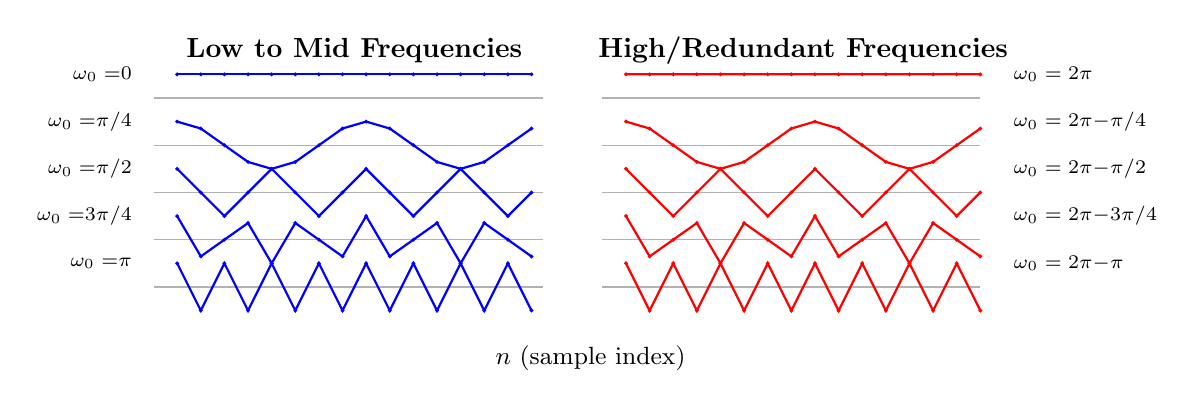
\begin{tikzpicture}[scale=0.3]
    % Settings for number of samples and axis
    \def\nmax{15}
    \def\rowsep{2}
    % Frequencies and labels
    \foreach \row/\freq/\label in {
        0/0/{$0$},
        1/{pi/4}/{$\pi/4$},
        2/{pi/2}/{$\pi/2$},
        3/{3*pi/4}/{$3\pi/4$},
        4/{pi}/{$\pi$}
    } {
        % Left column: 0 to pi
        % Draw x-axis
        \draw[gray!60] (-1, -\row*\rowsep) -- (\nmax+0.5, -\row*\rowsep);
        % Plot points and connect with lines
        \draw[blue, thick] (0, {cos(deg(\freq*0))-\row*\rowsep})
            \foreach \n in {1,...,\nmax} {
                -- (\n, {cos(deg(\freq*\n))-\row*\rowsep})
            };
        \foreach \n in {0,...,\nmax} {
            \pgfmathsetmacro{\y}{cos(deg(\freq*\n))}
            \filldraw[blue] (\n, \y-\row*\rowsep) circle (1.6pt);
        }
        \node[left] at (-1.5, 1-\row*\rowsep) {\scriptsize $\omega_0=$\label};

        % Right column: 2pi to pi
        \pgfmathsetmacro{\freqR}{2*pi-\freq}
        % Draw x-axis
        \draw[gray!60] (18, -\row*\rowsep) -- (18+\nmax+1, -\row*\rowsep);
        % Plot points and connect with lines
        \draw[red, thick] (19, {cos(deg(\freqR*0))-\row*\rowsep})
            \foreach \n in {1,...,\nmax} {
                -- (19+\n, {cos(deg(\freqR*\n))-\row*\rowsep})
            };
        \foreach \n in {0,...,\nmax} {
            \pgfmathsetmacro{\y}{cos(deg(\freqR*\n))}
            \filldraw[red] (19+\n, \y-\row*\rowsep) circle (1.6pt);
        }
        \ifnum\row=0
            \node[right] at (35, 1-\row*\rowsep) {\scriptsize $\omega_0=2\pi$};
        \else
            \node[right] at (35, 1-\row*\rowsep) {\scriptsize $\omega_0=2\pi-$\label};
        \fi
    }
    % Axis labels
    \node at (7.5, 2) {\textbf{Low to Mid Frequencies}};
    \node at (26.5, 2) {\textbf{High/Redundant Frequencies}};
    \node at (17.5, -11) {\small $n$ (sample index)};
\end{tikzpicture}
\end{center}
\vspace{0.5em}
{\footnotesize Each row compares signals with frequencies $\omega_0$ and $2\pi-\omega_0$. Blue and red lines connect the points of each sinusoid for better visibility.}
\end{frame}

\begin{frame}{Oscillation Rate vs. Frequency in Discrete-Time}
% \begin{center}
%     \includegraphics[width=0.7\linewidth]{figs/cos_omega_n.png}
% \end{center}
\begin{itemize}
    \item As $\omega_0$ increases from $0$ toward $\pi$, oscillations become more rapid.
    \item As $\omega_0$ increases from $\pi$ toward $2\pi$, oscillations slow down.
    \item Due to periodicity, $\omega_0 = 2\pi$ is identical to $\omega_0 = 0$.
\end{itemize}
\end{frame}



\begin{frame}{Summary: Discrete-Time Signals \& Systems}
\begin{itemize}
    \item \textbf{Signals:} Functions that convey information; can be continuous or discrete in time and amplitude.
    \item \textbf{Discrete-Time Signals:} Sequences $x[n]$, typically obtained by sampling a continuous signal.
    \item \textbf{Basic Sequences:} 
    \begin{itemize}
        \item Impulse ($\delta[n]$), step ($u[n]$), exponential, and sinusoidal sequences.
        \item Any sequence can be expressed as a sum of scaled, shifted impulses.
    \end{itemize}
    \item \textbf{Impulse and Step Relations:}
    \begin{itemize}
        \item $u[n]$ is the running sum of $\delta[n]$; $\delta[n]$ is the difference of $u[n]$.
    \end{itemize}
    \item \textbf{Sinusoids in Discrete Time:}
    \begin{itemize}
        \item Periodicity depends on frequency: only some discrete-time sinusoids are periodic.
        \item Frequencies separated by $2\pi$ are indistinguishable (aliasing effect).
        \item Only $N$ unique frequencies for period-$N$ sequences.
    \end{itemize}
    \item \textbf{Oscillation Rate:} Oscillation increases from $0$ to $\pi$; slows from $\pi$ to $2\pi$.
\end{itemize}

\end{frame}




% \begin{frame}{References}
% \begin{itemize}
%     \item \emph{Discrete-Time Signal Processing}, Oppenheim and Schafer, 3rd Edition (Section 2.1)
%     \item MIT OpenCourseWare: \url{https://ocw.mit.edu/}
% \end{itemize}
% \end{frame}





\end{document}
